% !TeX root = main.tex

% ============================================================
% thesis-sync entry: 2026-07-19_inchworm-smc-controller
% Type: design decision + numeric data (discrete-time SMC)
% Part of the INCHWORM ROBOT block (prior work, precedes the lizard sections).
% Insertable section block (no preamble). Requires: amsmath, graphicx.
% ============================================================

\section{PNEUMATIC SLIDING MODE CONTROLLER}
\label{sec:inchworm-smc}

The highly non-linear dynamics of compressible air, combined with the
asymmetric flow rates of active pumping versus passive venting, make
standard linear controllers (e.g., PID) difficult to tune across a wide
pressure range. To ensure robust tracking and stability, a discrete-time
Sliding Mode Controller (SMC) was implemented for each of the eight
independent channels.

The primary objective of the controller is to drive the pressure error,
$e(t) = P_{\text{target}} - P_{\text{actual}}$, and its time derivative,
$\dot{e}(t)$, to zero. A time-varying sliding surface, $s(t)$, is defined in
the phase plane as:
\begin{equation}
s(t) = \lambda_1 e(t) + \lambda_2 \dot{e}(t)
\label{eq:inchworm-sliding_surface}
\end{equation}
where $\lambda_1 > 0$ and $\lambda_2 > 0$ are tuning parameters that
respectively dictate the convergence rate of the error trajectory and the
damping of the error dynamics. The ideal control law would constrain the
system state to $s(t) = 0$. However, standard SMC relies on high-frequency
discontinuous switching across the sliding surface, which in a discrete
pneumatic system leads to severe solenoid valve chattering, accelerating
mechanical wear.

To mitigate this, a boundary-layer approach was adopted by introducing a
saturation function bounded by a width parameter, $\Phi$. The normalized
control effort, $u(t)$, is defined as:
\begin{equation}
u(t) = \text{sat}\!\left(\frac{s(t)}{\Phi}\right)
\label{eq:inchworm-control_effort}
\end{equation}
where $\text{sat}(x)$ maps the input to the range $[-1, 1]$. This establishes
a boundary layer ($|s| \le \Phi$) in which the control action becomes more
refined, smoothing the actuator response as the pressure approaches the
target.

Because the system uses strictly on/off solenoid valves, the control effort
$u(t)$ is translated into a Pulse-Width Modulated (PWM) signal. The active
duration of the valve opening for a given control cycle, $t_{\text{pulse}}$,
is calculated as:
\begin{equation}
t_{\text{pulse}} = |u(t)| \cdot K_{\text{gain}}
\label{eq:inchworm-pulse_width}
\end{equation}
where $K_{\text{gain}}$ represents the maximum allowable pulse duration.

To optimize energy efficiency and increase control resolution near the
target pressure, an asymmetric actuation strategy was incorporated. The sign
of $u(t)$ determines the direction of airflow (inflation for $u > 0$,
deflation for $u < 0$). During deflation, the controller assesses the
magnitude of the control effort and the current chamber pressure. If the
required effort is small ($|u(t)| < 0.4$) and the chamber pressure is above
atmospheric pressure, the controller enters a ``passive venting'' mode. In
this state, the exhaust valve is opened while the shared vacuum pump remains
disabled, allowing ambient pressure equalization to gently deflate the
chamber. To compensate for the diminishing pressure gradient during passive
venting, the pulse duration $t_{\text{pulse}}$ is dynamically scaled
inversely proportional to the current chamber pressure. For higher control
efforts ($|u(t)| \ge 0.4$) or when drawing negative gauge pressure, the
system engages active vacuum deflation. Fig.~\ref{fig:inchworm-stepresponse}
shows the controller's step response.

\begin{figure}[tbh]
 \centering
  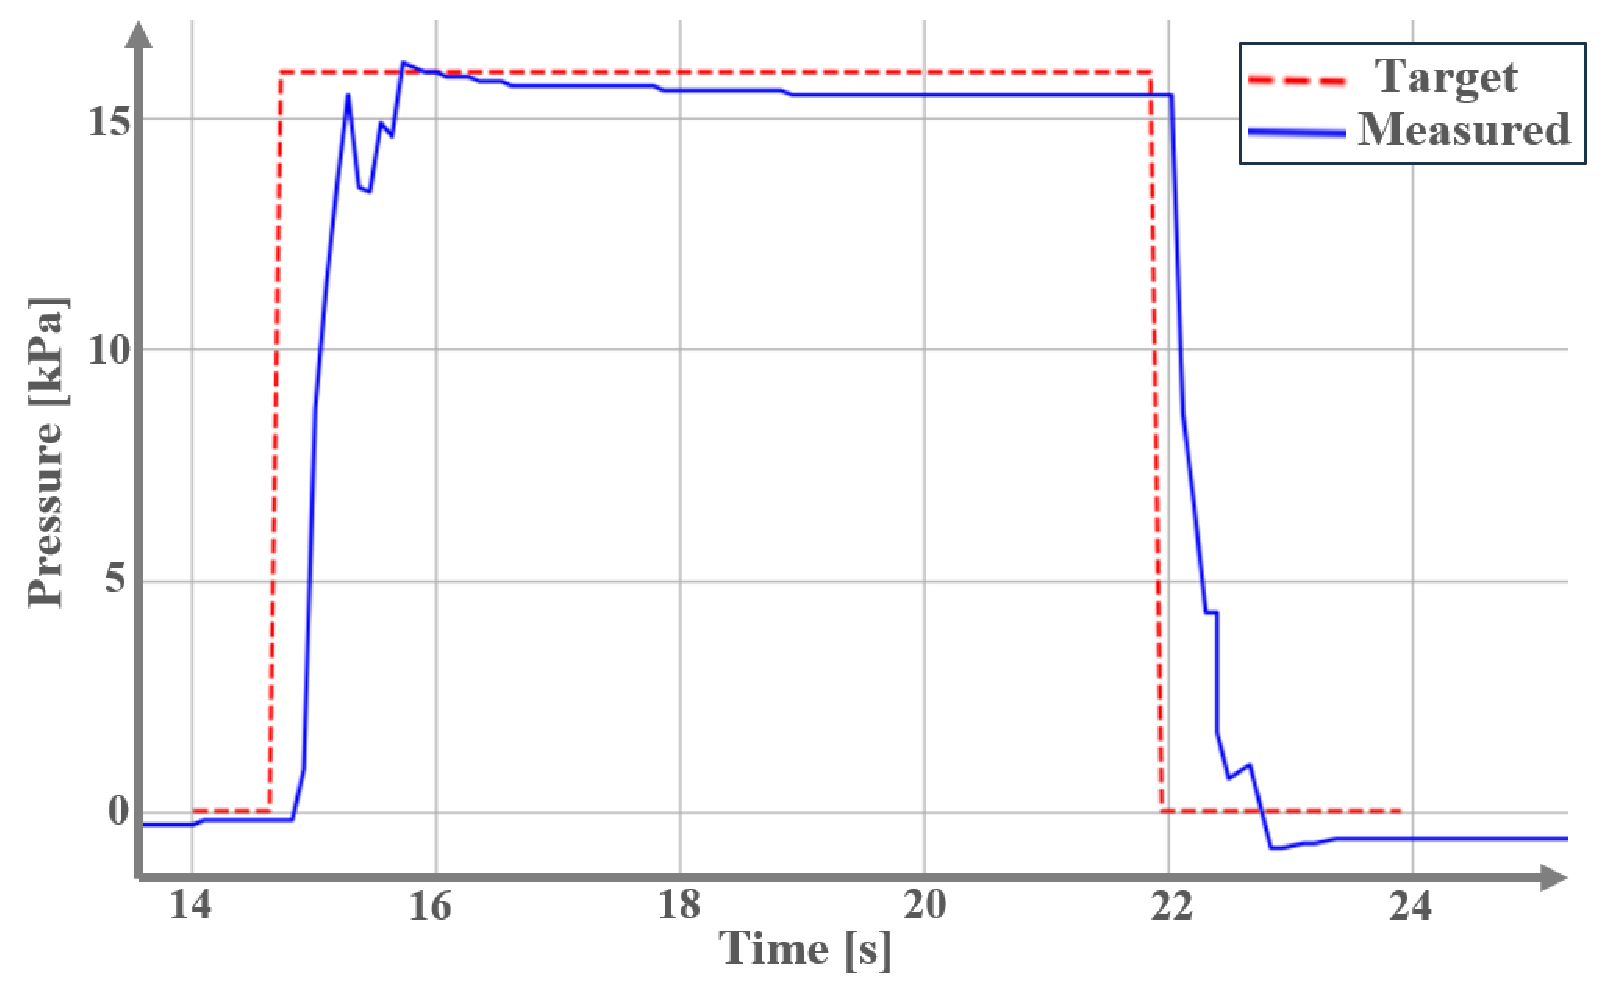
\includegraphics[height=40mm]{figures/stepresponse.eps}
  \vspace*{-2mm}
  \caption{Step response of the pneumatic system sliding mode controller.}
  \label{fig:inchworm-stepresponse}
\end{figure}

Finally, while the eight independent channels asynchronously compute their
control inputs, a centralized pump manager monitors their states. If any
single channel dictates an active inflation or deflation pulse exceeding the
hardware threshold ($t_{\text{pulse}} > 30$~ms), the respective shared pump
is engaged.
